\PassOptionsToPackage{unicode=true}{hyperref} % options for packages loaded elsewhere
\PassOptionsToPackage{hyphens}{url}
%
\documentclass[ignorenonframetext,]{beamer}
\usepackage{pgfpages}
\setbeamertemplate{caption}[numbered]
\setbeamertemplate{caption label separator}{: }
\setbeamercolor{caption name}{fg=normal text.fg}
\beamertemplatenavigationsymbolsempty
\usepackage{lmodern}
\usepackage{amssymb,amsmath}
\usepackage{ifxetex,ifluatex}
\usepackage{fixltx2e} % provides \textsubscript
\ifnum 0\ifxetex 1\fi\ifluatex 1\fi=0 % if pdftex
  \usepackage[T1]{fontenc}
  \usepackage[utf8]{inputenc}
  \usepackage{textcomp} % provides euro and other symbols
\else % if luatex or xelatex
  \usepackage{unicode-math}
  \defaultfontfeatures{Ligatures=TeX,Scale=MatchLowercase}
\fi
\usetheme[]{CambridgeUS}
\usecolortheme{beaver}
\usefonttheme{structurebold}
% use upquote if available, for straight quotes in verbatim environments
\IfFileExists{upquote.sty}{\usepackage{upquote}}{}
% use microtype if available
\IfFileExists{microtype.sty}{%
\usepackage[]{microtype}
\UseMicrotypeSet[protrusion]{basicmath} % disable protrusion for tt fonts
}{}
\IfFileExists{parskip.sty}{%
\usepackage{parskip}
}{% else
\setlength{\parindent}{0pt}
\setlength{\parskip}{6pt plus 2pt minus 1pt}
}
\usepackage{hyperref}
\hypersetup{
            pdftitle={Daten beschaffen},
            pdfauthor={Jan-Philipp Kolb},
            pdfborder={0 0 0},
            breaklinks=true}
\urlstyle{same}  % don't use monospace font for urls
\newif\ifbibliography
\usepackage{color}
\usepackage{fancyvrb}
\newcommand{\VerbBar}{|}
\newcommand{\VERB}{\Verb[commandchars=\\\{\}]}
\DefineVerbatimEnvironment{Highlighting}{Verbatim}{commandchars=\\\{\}}
% Add ',fontsize=\small' for more characters per line
\usepackage{framed}
\definecolor{shadecolor}{RGB}{42,33,28}
\newenvironment{Shaded}{\begin{snugshade}}{\end{snugshade}}
\newcommand{\AlertTok}[1]{\textcolor[rgb]{1.00,1.00,0.00}{#1}}
\newcommand{\AnnotationTok}[1]{\textcolor[rgb]{0.00,0.40,1.00}{\textbf{\textit{#1}}}}
\newcommand{\AttributeTok}[1]{\textcolor[rgb]{0.74,0.68,0.62}{#1}}
\newcommand{\BaseNTok}[1]{\textcolor[rgb]{0.27,0.67,0.26}{#1}}
\newcommand{\BuiltInTok}[1]{\textcolor[rgb]{0.74,0.68,0.62}{#1}}
\newcommand{\CharTok}[1]{\textcolor[rgb]{0.02,0.61,0.04}{#1}}
\newcommand{\CommentTok}[1]{\textcolor[rgb]{0.00,0.40,1.00}{\textbf{\textit{#1}}}}
\newcommand{\CommentVarTok}[1]{\textcolor[rgb]{0.74,0.68,0.62}{#1}}
\newcommand{\ConstantTok}[1]{\textcolor[rgb]{0.74,0.68,0.62}{#1}}
\newcommand{\ControlFlowTok}[1]{\textcolor[rgb]{0.26,0.66,0.93}{\textbf{#1}}}
\newcommand{\DataTypeTok}[1]{\textcolor[rgb]{0.74,0.68,0.62}{\underline{#1}}}
\newcommand{\DecValTok}[1]{\textcolor[rgb]{0.27,0.67,0.26}{#1}}
\newcommand{\DocumentationTok}[1]{\textcolor[rgb]{0.00,0.40,1.00}{\textit{#1}}}
\newcommand{\ErrorTok}[1]{\textcolor[rgb]{1.00,1.00,0.00}{\textbf{#1}}}
\newcommand{\ExtensionTok}[1]{\textcolor[rgb]{0.74,0.68,0.62}{#1}}
\newcommand{\FloatTok}[1]{\textcolor[rgb]{0.27,0.67,0.26}{#1}}
\newcommand{\FunctionTok}[1]{\textcolor[rgb]{1.00,0.58,0.35}{\textbf{#1}}}
\newcommand{\ImportTok}[1]{\textcolor[rgb]{0.74,0.68,0.62}{#1}}
\newcommand{\InformationTok}[1]{\textcolor[rgb]{0.00,0.40,1.00}{\textbf{\textit{#1}}}}
\newcommand{\KeywordTok}[1]{\textcolor[rgb]{0.26,0.66,0.93}{\textbf{#1}}}
\newcommand{\NormalTok}[1]{\textcolor[rgb]{0.74,0.68,0.62}{#1}}
\newcommand{\OperatorTok}[1]{\textcolor[rgb]{0.74,0.68,0.62}{#1}}
\newcommand{\OtherTok}[1]{\textcolor[rgb]{0.74,0.68,0.62}{#1}}
\newcommand{\PreprocessorTok}[1]{\textcolor[rgb]{0.74,0.68,0.62}{\textbf{#1}}}
\newcommand{\RegionMarkerTok}[1]{\textcolor[rgb]{0.74,0.68,0.62}{#1}}
\newcommand{\SpecialCharTok}[1]{\textcolor[rgb]{0.02,0.61,0.04}{#1}}
\newcommand{\SpecialStringTok}[1]{\textcolor[rgb]{0.02,0.61,0.04}{#1}}
\newcommand{\StringTok}[1]{\textcolor[rgb]{0.02,0.61,0.04}{#1}}
\newcommand{\VariableTok}[1]{\textcolor[rgb]{0.74,0.68,0.62}{#1}}
\newcommand{\VerbatimStringTok}[1]{\textcolor[rgb]{0.02,0.61,0.04}{#1}}
\newcommand{\WarningTok}[1]{\textcolor[rgb]{1.00,1.00,0.00}{\textbf{#1}}}
\usepackage{longtable,booktabs}
\usepackage{caption}
% These lines are needed to make table captions work with longtable:
\makeatletter
\def\fnum@table{\tablename~\thetable}
\makeatother
\usepackage{graphicx,grffile}
\makeatletter
\def\maxwidth{\ifdim\Gin@nat@width>\linewidth\linewidth\else\Gin@nat@width\fi}
\def\maxheight{\ifdim\Gin@nat@height>\textheight\textheight\else\Gin@nat@height\fi}
\makeatother
% Scale images if necessary, so that they will not overflow the page
% margins by default, and it is still possible to overwrite the defaults
% using explicit options in \includegraphics[width, height, ...]{}
\setkeys{Gin}{width=\maxwidth,height=\maxheight,keepaspectratio}
% Prevent slide breaks in the middle of a paragraph:
\widowpenalties 1 10000
\raggedbottom
\setbeamertemplate{part page}{
\centering
\begin{beamercolorbox}[sep=16pt,center]{part title}
  \usebeamerfont{part title}\insertpart\par
\end{beamercolorbox}
}
\setbeamertemplate{section page}{
\centering
\begin{beamercolorbox}[sep=12pt,center]{part title}
  \usebeamerfont{section title}\insertsection\par
\end{beamercolorbox}
}
\setbeamertemplate{subsection page}{
\centering
\begin{beamercolorbox}[sep=8pt,center]{part title}
  \usebeamerfont{subsection title}\insertsubsection\par
\end{beamercolorbox}
}
\AtBeginPart{
  \frame{\partpage}
}
\AtBeginSection{
  \ifbibliography
  \else
    \frame{\sectionpage}
  \fi
}
\AtBeginSubsection{
  \frame{\subsectionpage}
}
\setlength{\emergencystretch}{3em}  % prevent overfull lines
\providecommand{\tightlist}{%
  \setlength{\itemsep}{0pt}\setlength{\parskip}{0pt}}
\setcounter{secnumdepth}{0}

% set default figure placement to htbp
\makeatletter
\def\fps@figure{htbp}
\makeatother


\title{Daten beschaffen}
\author{Jan-Philipp Kolb}
\date{22 Oktober 2018}

\begin{document}
\frame{\titlepage}

\begin{frame}

\end{frame}

\begin{frame}{\href{http://inspire.ec.europa.eu/reports/Registration_form.pdf}{EU
Initiative INSPIRE}}
\protect\hypertarget{eu-initiative-inspire}{}


\includegraphics{figure/inspire.PNG}

\begin{block}{Ziele:}

\begin{itemize}
\tightlist
\item
  Räumliche Information zugänglicher und interoperabel machen
\item
  Nachhaltige Entwicklung in diesem Bereich unterstützen
\end{itemize}

\end{block}

\begin{block}{Entwicklung}

\begin{itemize}
\tightlist
\item
  Aufgrund der Richtlinie sind mehr Daten frei verfügbar.
\end{itemize}

\end{block}

\end{frame}

\begin{frame}{Zensus Atlas}
\protect\hypertarget{zensus-atlas}{}

Für den Zensus 2011 kann man Daten herunterladen und/oder diese in
Karten visualisieren.

\begin{block}{\url{https://ergebnisse.zensus2011.de/}}

\begin{figure}
\centering
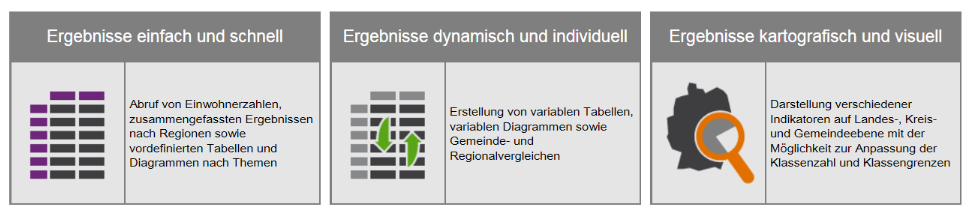
\includegraphics{figure/Zensusdtb.PNG}
\caption{Zensus Datenbank}
\end{figure}

\end{block}

\end{frame}

\begin{frame}{\href{https://www.destatis.de/DE/Methoden/Zensus_/Zensus.html}{Zensus
Gemeindeergebnisse}}
\protect\hypertarget{zensus-gemeindeergebnisse}{}

\includegraphics{figure/ZensusMigbg.PNG}

\end{frame}

\begin{frame}{A3A Aufgabe: Zensus Ergebnisse für Gemeinden downloaden}
\protect\hypertarget{a3a-aufgabe-zensus-ergebnisse-fur-gemeinden-downloaden}{}

\begin{itemize}
\tightlist
\item
  Lade die Zensus Gemeinde Ergebnisse
  \href{https://www.zensus2011.de/SharedDocs/Aktuelles/Ergebnisse/DemografischeGrunddaten.html}{\textbf{hier}}
  herunter.
\item
  Importiere die Daten mit einer geeigneten Funktion in R.
\item
  Welche Information ist in den Daten enthalten?
\end{itemize}

\end{frame}

\begin{frame}{\href{https://de.wikipedia.org/wiki/Amtlicher_Gemeindeschl\%C3\%BCssel}{Der
amtliche Gemeindeschlüssel}}
\protect\hypertarget{der-amtliche-gemeindeschlussel}{}

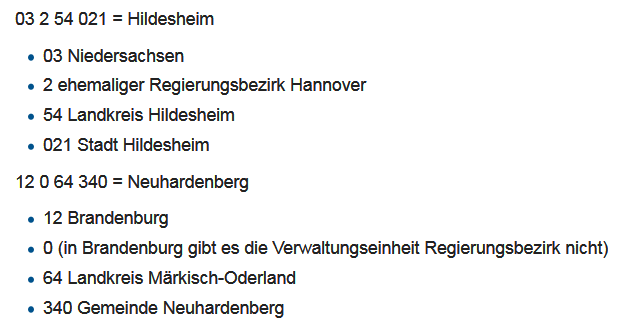
\includegraphics{figure/ags_beispiele.PNG}

\end{frame}

\begin{frame}{AGS - Bundesländer}
\protect\hypertarget{ags---bundeslander}{}

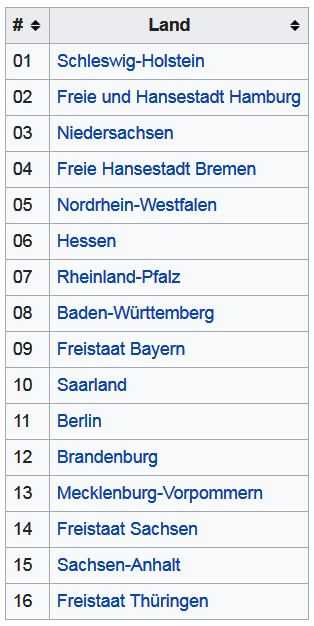
\includegraphics{figure/AGS_BLA.PNG}

\end{frame}

\begin{frame}{A3B Aufgabe}
\protect\hypertarget{a3b-aufgabe}{}

\begin{itemize}
\tightlist
\item
  Nutze die Gemeindeergebnisse für den Zensus 2011 und erzeuge einen
  Datensatz, der nur die Ergebnisse für die Saarländischen Gemeinden
  enthält.
\item
  Ermittle aus diesem Datensatz die Gemeinde in der der Anteil der unter
  1-jährigen am höchsten ist.
\item
  Speichere einen Datensatz ab, in dem die folgenden Variablen enthalten
  sind:

  \begin{itemize}
  \tightlist
  \item
    der amtliche Gemeindeschlüssel,
  \item
    die Gemeindenamen,\\
  \item
    die Bevölkerungszahl insgesamt
  \item
    die Zahl der Einjährigen und
  \item
    die Zahl der Zwanzigjährigen
  \end{itemize}
\end{itemize}

\end{frame}

\begin{frame}{Forschungsdatenzentren}
\protect\hypertarget{forschungsdatenzentren}{}

\begin{itemize}
\tightlist
\item
  Bspw. FDZ der statistischen Ämter:
\end{itemize}

\url{http://www.forschungsdatenzentrum.de/}

\begin{itemize}
\item
  Es werden hauptsächlich Public Use Files angeboten,
\item
  Teilweise können Gewichtungsfaktoren verwendet werden um regionale
  Ergebnisse zu bekommen
\item
  In der Regel ist Darstellung in Karten aber schwierig
\end{itemize}

\end{frame}

\begin{frame}{Weitere Amtliche Datenquellen}
\protect\hypertarget{weitere-amtliche-datenquellen}{}

\begin{itemize}
\item
  Die Regionaldatenbank
  \href{https://www-genesis.destatis.de/genesis/online}{\textbf{Genesis}}
\item
  Daneben gibt es Angebote der Landesämter bspw das Angebot des
  \href{https://www.statistik.rlp.de/regionaldaten/}{\textbf{statistischen
  Landesamts Rheinland-Pfalz}}
\end{itemize}

\end{frame}

\begin{frame}[fragile]{Eurostat Daten}
\protect\hypertarget{eurostat-daten}{}

\begin{block}{Beispiel: Principal European Economic Indicators}

\url{http://ec.europa.eu/eurostat/web/euro-indicators/peeis}

\begin{Shaded}
\begin{Highlighting}[]
\KeywordTok{library}\NormalTok{(xlsx)}
\NormalTok{HHsr <-}\StringTok{ }\KeywordTok{read.xlsx2}\NormalTok{(}\KeywordTok{paste0}\NormalTok{(eurostatpath,}\StringTok{"HHsavingRate.xls"}\NormalTok{),}\DecValTok{1}\NormalTok{)}
\end{Highlighting}
\end{Shaded}

\begin{longtable}[]{@{}lllll@{}}
\toprule
geo & X2012Q3 & X2012Q4 & X2013Q1 & X2013Q2\tabularnewline
\midrule
\endhead
Euro area (19 countries) & 9.82 & 11.86 & 11.37 & 16.28\tabularnewline
EU (28 countries) & 8.67 & 10.92 & 9.42 & 14.63\tabularnewline
Belgium & 12.52 & 9.33 & 13.99 & 19.03\tabularnewline
Czech Republic & 10.16 & 14.81 & 9.46 & 10.44\tabularnewline
\bottomrule
\end{longtable}

\end{block}

\end{frame}

\begin{frame}{A3A Übung: Download von Eurostat Daten}
\protect\hypertarget{a3a-ubung-download-von-eurostat-daten}{}

\begin{itemize}
\tightlist
\item
  Gehe auf die Website mit den \emph{Principal European Economic
  Indicators} und lade die Statistik der Sparquote
  \href{http://ec.europa.eu/eurostat/web/euro-indicators/peeis}{\textbf{hier}}
  herunter.
\item
  Importiere die Daten in R mit einem geeigneten Befehl.
\end{itemize}

\end{frame}

\begin{frame}{Daten - Institut für ökologische Raumforschung (IÖR)}
\protect\hypertarget{daten---institut-fur-okologische-raumforschung-ior}{}

\includegraphics{figure/ioerMonitor.PNG}

\begin{itemize}
\tightlist
\item
  Hier gibt es bspw. Indikatoren zu Nachhaltigkeit, Siedlung, Gebäuden,
  Verkehr etc.
\item
  Es könnte also interessant sein, diese Daten an das Gesis Panel
  anzuspielen
\item
  Aber dazu später mehr
\end{itemize}

\end{frame}

\begin{frame}{Datahub.io}
\protect\hypertarget{datahub.io}{}

\begin{itemize}
\tightlist
\item
  Auf dieser Plattform sind sehr viele Daten vorhanden,
\item
  bspw. der UNESCO
  \href{http://datahub.io/dataset/unesco-world-heritage-sites/resource/d4116195-44d8-4bc1-9f91-9b570870dc19}{\textbf{Weltkulturerbe}}
  Datensatz, den ich in der Folge auch in Beispielen verwenden werde.
\end{itemize}

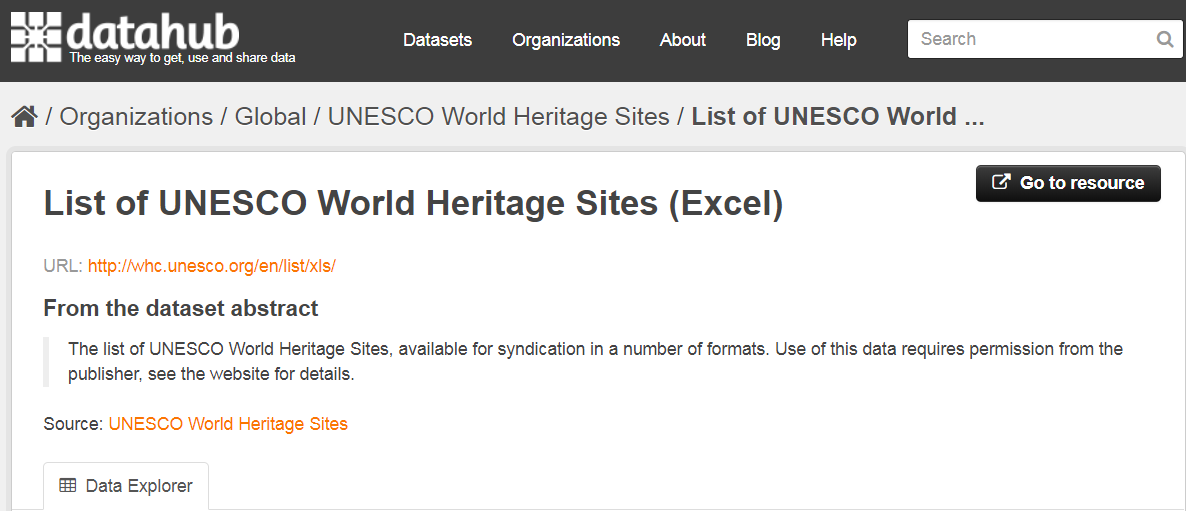
\includegraphics{figure/datahub_whc.PNG}

\begin{longtable}[]{@{}llrrl@{}}
\toprule
& name\_en & longitude & latitude & category\_short\tabularnewline
\midrule
\endhead
4 & Butrint & 20.03 & 39.75 & C\tabularnewline
5 & Al Qal'a of Beni Hammad & 4.79 & 35.82 & C\tabularnewline
6 & M'Zab Valley & 3.68 & 32.48 & C\tabularnewline
7 & Djémila & 5.74 & 36.32 & C\tabularnewline
8 & Timgad & 6.63 & 35.45 & C\tabularnewline
\bottomrule
\end{longtable}

\end{frame}

\begin{frame}{American Community Survey}
\protect\hypertarget{american-community-survey}{}

\begin{block}{\href{http://www.census.gov/acs/www/}{Die Daten des
\emph{American Community Survey:}}}

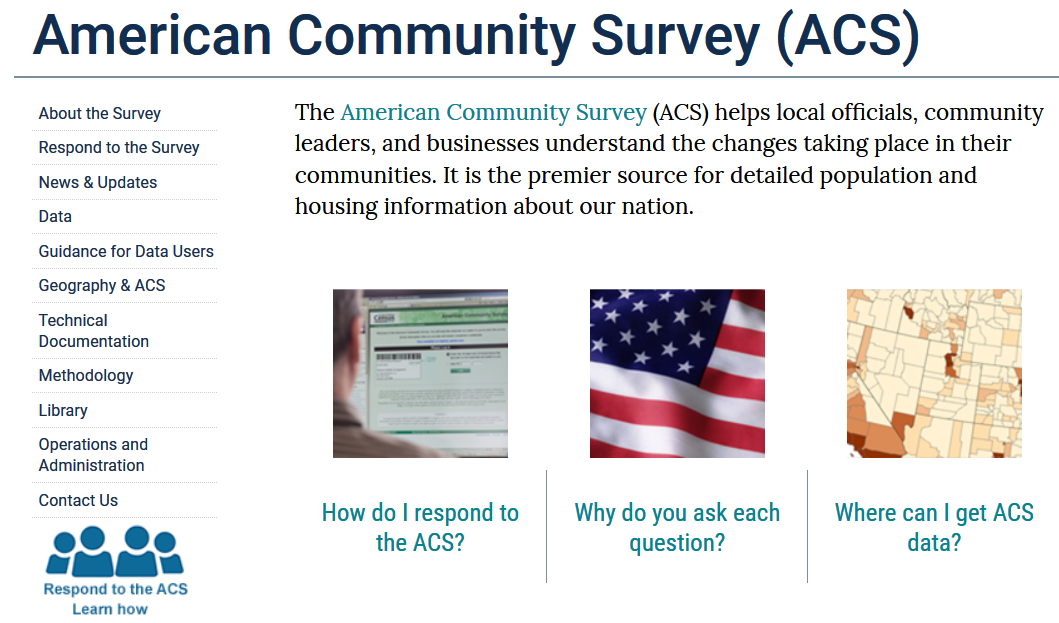
\includegraphics{figure/ACS.PNG}

\end{block}

\end{frame}

\begin{frame}{\href{data.hdx.rwlabs.org}{The Humanitarian Data
Exchange}}
\protect\hypertarget{the-humanitarian-data-exchange}{}

\begin{block}{Zum Beispiel Daten zur
\href{https://data.hdx.rwlabs.org/dataset/rowca-ebola-cases}{Ebola
Epedemie}}

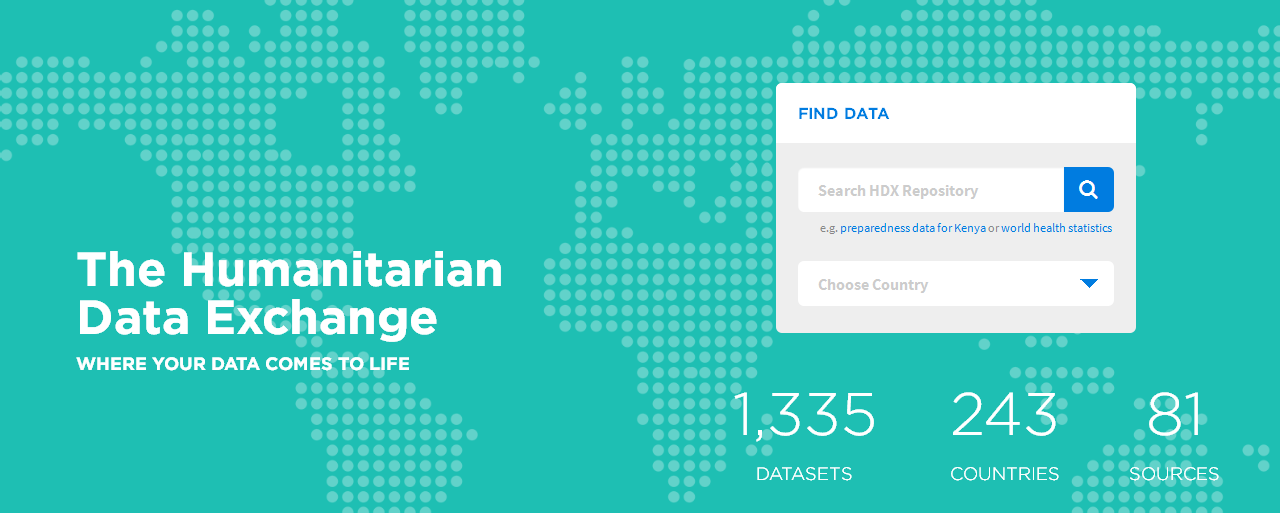
\includegraphics{figure/HDx.PNG}

\end{block}

\end{frame}

\begin{frame}[fragile]{Weltbank Daten}
\protect\hypertarget{weltbank-daten}{}

\begin{itemize}
\tightlist
\item
  AG.AGR.TRAC.NO -
  \href{https://data.worldbank.org/indicator/AG.AGR.TRAC.NO}{\textbf{Agricultural
  machinery, tractors}}
\end{itemize}

\begin{Shaded}
\begin{Highlighting}[]
\KeywordTok{library}\NormalTok{(WDI) }
\NormalTok{WDI_dat <-}\StringTok{ }\KeywordTok{WDI}\NormalTok{(}\DataTypeTok{country=}\StringTok{"all"}\NormalTok{,}
    \DataTypeTok{indicator=}\KeywordTok{c}\NormalTok{(}\StringTok{"AG.AGR.TRAC.NO"}\NormalTok{,}
    \StringTok{"TM.TAX.TCOM.BC.ZS"}\NormalTok{),}
    \DataTypeTok{start=}\DecValTok{1990}\NormalTok{, }\DataTypeTok{end=}\DecValTok{2000}\NormalTok{)}
\end{Highlighting}
\end{Shaded}

\begin{itemize}
\tightlist
\item
  Es gibt auch eine Funktion \texttt{WDIsearch} mit der man nach
  Indikatoren suchen kann
\end{itemize}

\begin{Shaded}
\begin{Highlighting}[]
\KeywordTok{head}\NormalTok{(WDI_dat)}
\end{Highlighting}
\end{Shaded}

\end{frame}

\begin{frame}{\href{http://data.london.gov.uk/dataset}{London
Datastore}}
\protect\hypertarget{london-datastore}{}

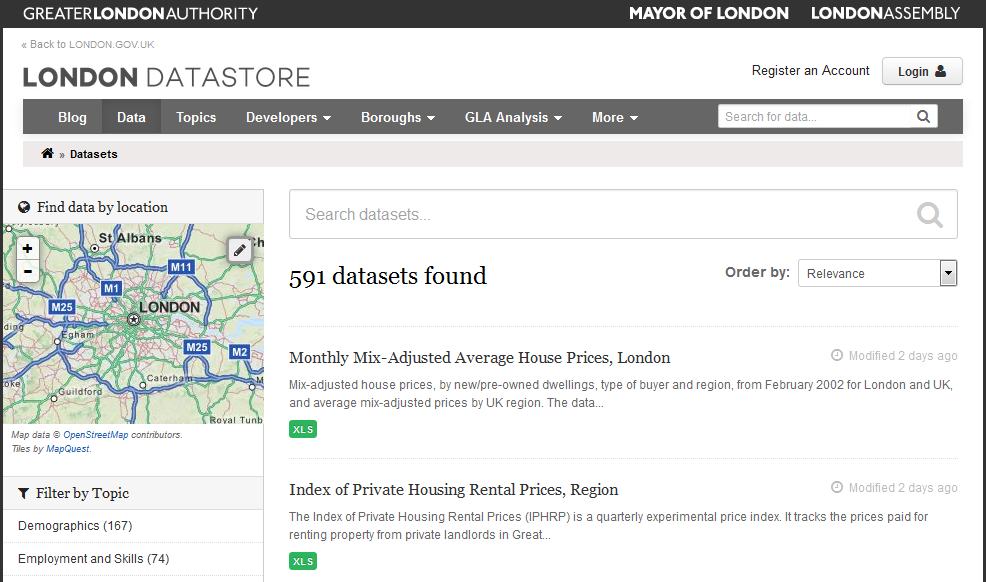
\includegraphics{figure/LondonData.PNG}

\end{frame}

\begin{frame}{Ein Beispieldatensatz für London}
\protect\hypertarget{ein-beispieldatensatz-fur-london}{}

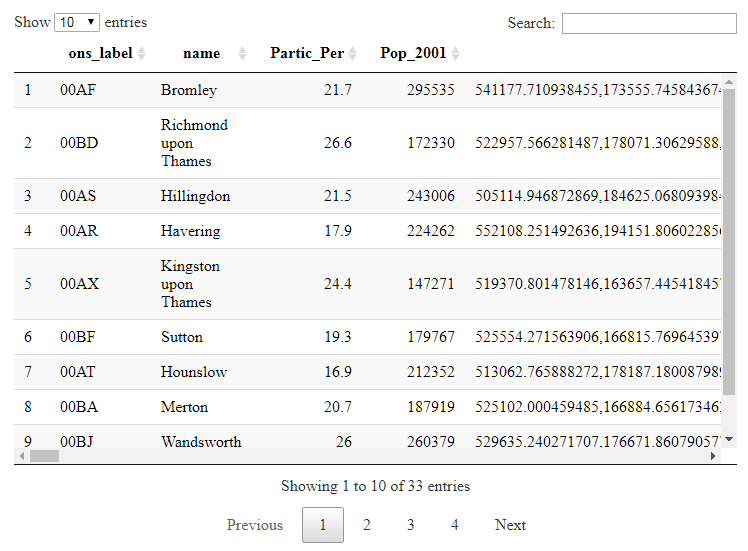
\includegraphics{figure/LondonExample.PNG}

\end{frame}

\end{document}
